\documentclass[12pt]{scrbook}

\usepackage{geometry}
\usepackage{graphicx}

\graphicspath{ {./images/} }

\geometry{
    a5paper
}

\begin{document}
\title{Dragon Rock}
\subtitle{A fantasy role playing game for the Commodore C65 series of computers}
\author{7Turtles Software}
\maketitle

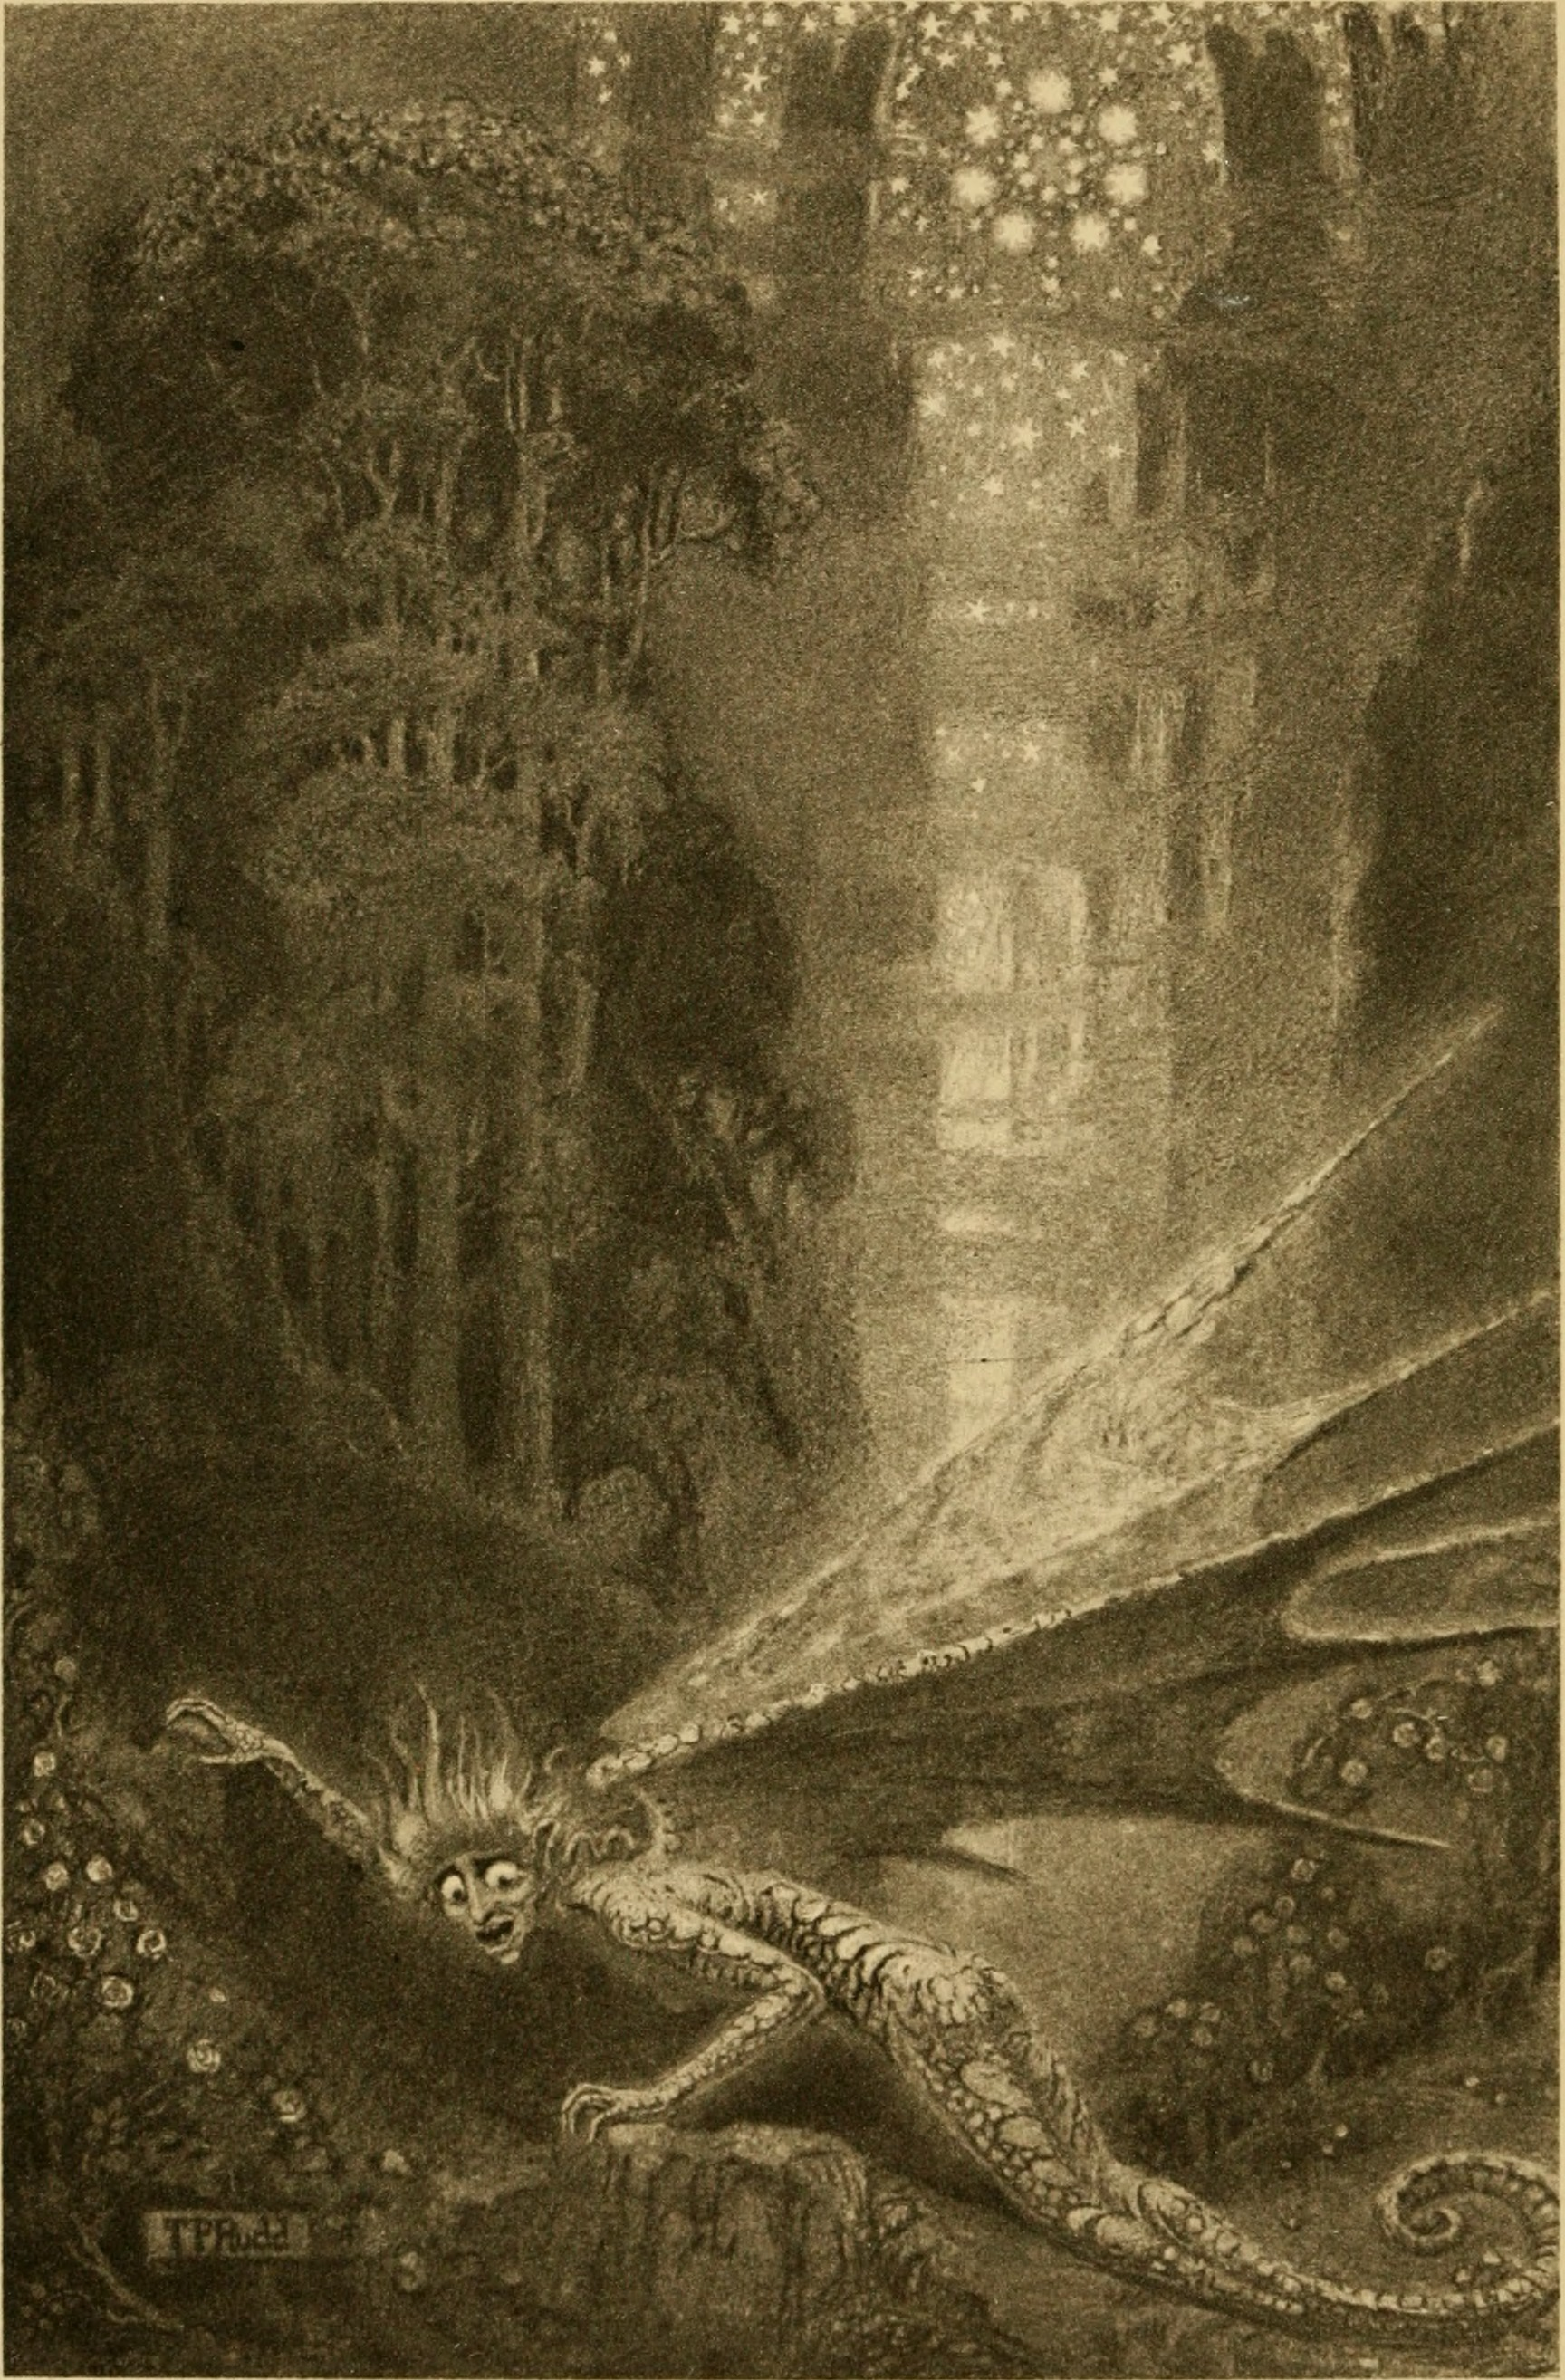
\includegraphics[width=\textwidth]{illustrations/ddungeon}


\chapter*{The story so far\dots}

For the longest time, everything seemed to be going just right in the Tianad province. People were happy - perhaps they even were the happiest people in all of the great kingdom of Narcordia.

And why wouldn't they?

The summers were warm and winters mild, harvest had been great and plentiful for years on end now, commerce was flourishing, the roads were reasonably secure, almost every citizen of Tianad had enough to eat and drink and a roof over their heads... it really seemed as if the gods were smiling down on the little province on the southeast border of Nacordia.

The change came slowly. At first, no one really noticed how fewer and fewer merchants from foreign lands were to be seen in the five major cities of Tianad. But then, as food and drink got scarce, stories of people disappearing from the roads at night were told in hushed voices in Tianads ever less frequented inns.

Then the raids started. Troops of all kinds of monsters and thieves started paying regular visits to many of the smaller villages of Tianad, stealing and pillaging from merchants and private homes alike.

Even the weather seemed to change -- summers grew hotter and hotter, torrential rains in autumn washed away the dried up ground, and winters were bitter and deadly cold.

For some time, people still hoped that the king would send reinforcements from his Dragon Guard to get the situation under control -- but reinforcements never came, and the few and in between remaining dragon guard soldiers stationed in Tianad soon disappeared.

\medskip

But amidst the resignation and fear, there's still hope. Adventurers of all professions gather in the guilds and inns all over Tianad, wondering what can be done about the situation. Wondering why there is no word from the borders. Wondering what happened to the king's Dragon Guard. Wondering where the monster gangs are coming from.

And now, there's a rumour going around that in the remote city of Foxhome, a band of brave and intrepid adventurers has gathered to head off and find answers to all of these questions\dots and to save the once prosperous province of Tianad.

\chapter{Introduction}
Thank you very much for purchasing \textit{Dragon Rock}. We hope that you have as much fun playing as we had creating it. In order to have the best possible experience, please read this manual carefully.

\section*{How to read this manual}

This manual has been provided for beginners and experienced users alike. If you have no idea what computer role playing gaming is about, you're encouraged to read the entire manual. 

\begin{figure}[ht]
    \centering
    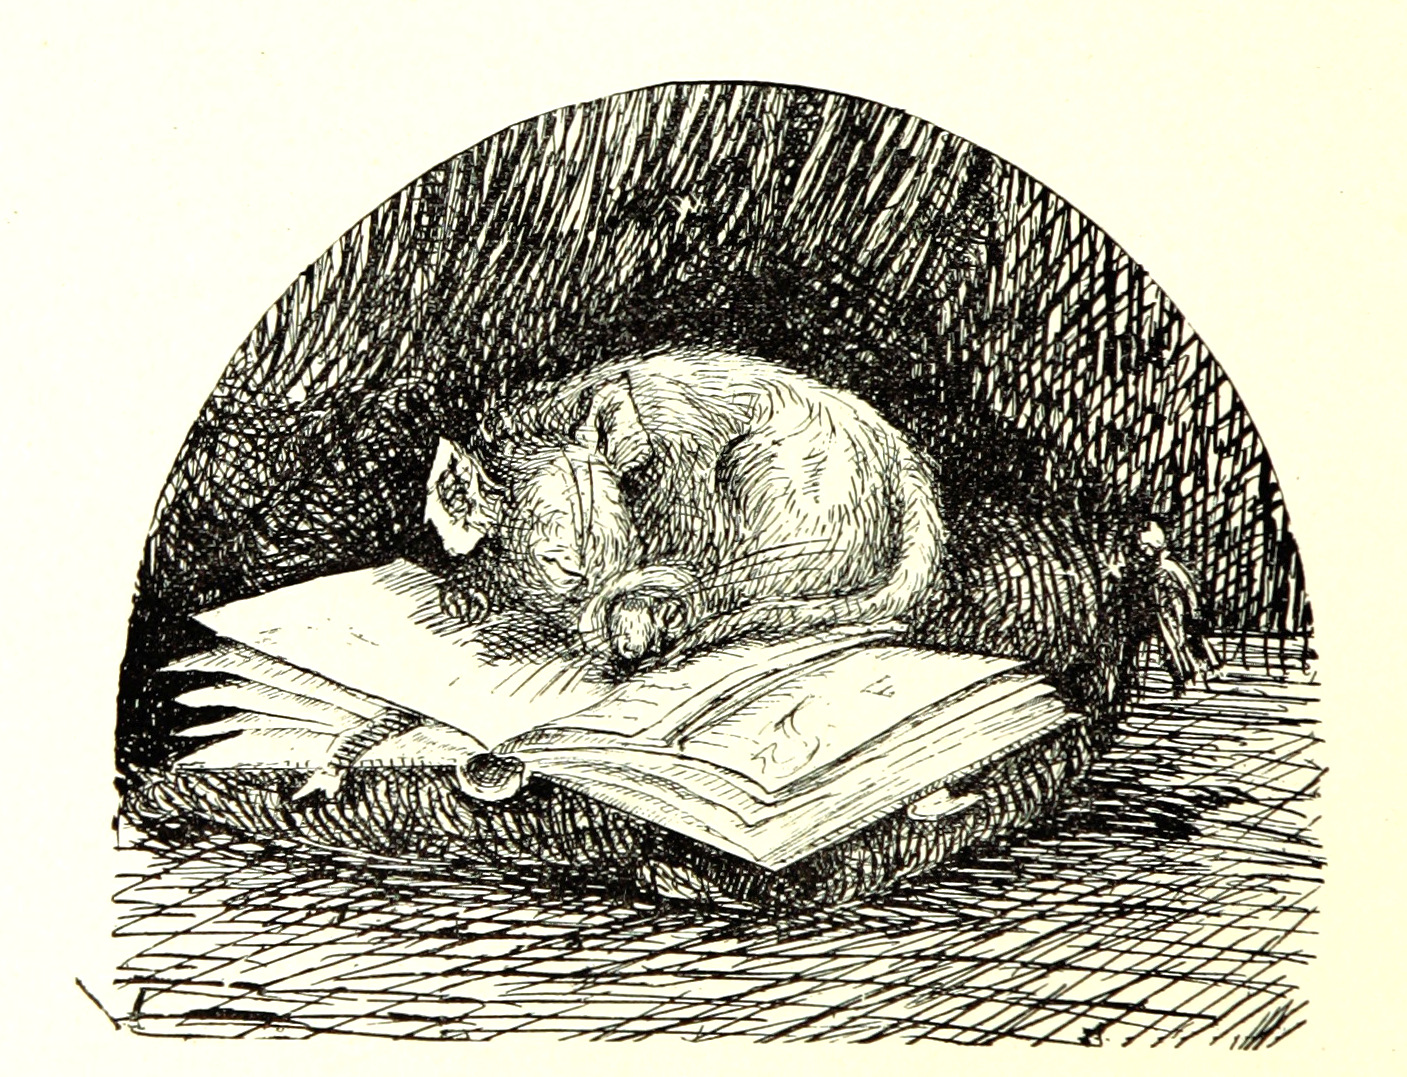
\includegraphics[width=0.5\textwidth]{illustrations/dormouse.jpg}
\end{figure}

If you have previous experience with computer role playing games, you may skip chapters two and three and instead begin directly with chapter 4. 


\section*{Requirements}
\textit{Dragon Rock} is a fantasy role plaiyng game designed for the Commodore \textit{C65} series of computers. In order to run \textit{Dragon Rock}, you will need the following:
\begin{itemize}
    \item A Commodore C65 or MEGA65 computer with \textbf{128K of RAM}. Please note that the game makes use of the C65s advanced features and therefore will not work on an ordinary C64.
    \item A Commodore 1581 or compatible drive.
    \item A monochrome or -- recommended -- colour monitor.
\end{itemize}

\section*{Before you start}
Before starting your journey through Tianad, please do take the time and make a backup of the supplied game disc.

\section*{If things go wrong}
A lot of time and effort went into the creation of \textit{Dragon Rock}. Nevertheless we can't be sure that the game is entirely bug-free. Should you happen to stumble upon an error in the game (or get stuck in any other way), please contact us at \texttt{dr@7turtles.de}


\chapter{How to play}

\section*{Starting the game}
To start the game, power up your computer and disc drive, insert the Dragon Rock Program Disc into the drive and type
\begin{verbatim}
BOOT
\end{verbatim}
followed by the \texttt{RETURN} key. After the file has loaded successfully and the computer displays \texttt{READY}, type in
\begin{verbatim}
RUN
\end{verbatim}
again followed by the \texttt{RETURN} key to start the game.

\section*{Setting up a party}
On the first screen of the game, you're given the choice to either load a saved game or start in the village of Foxhome:

\begin{figure}[ht]
    \centering
    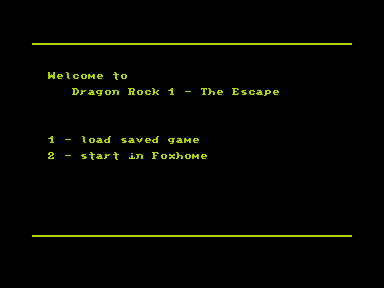
\includegraphics[width=0.5\textwidth]{startscreen}
    \caption{Start screen}
\end{figure}

Since you'll have no saved game in the beginning, choose \textbf{option number two}\footnote{It doesn't actually matter which option you choose at this point; both options will place you in Foxhome with an empty party roster} to enter Foxhome. After a short time of loading, you will be presented with the following screen:

\begin{figure}[ht]
    \centering
    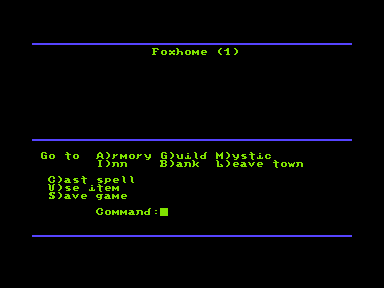
\includegraphics[width=0.5\textwidth]{emptyCity}
    \caption{Starting in Foxhome}
\end{figure}

The empty area in the upper half of the screen is the space where the individual members of your party are listed. Since you have no party as of yet, this space remains empty.

The city\footnote{Foxhome is one of Tianads seven major villages. While most services, such as the Adventurers' Guild, the Armory and the Inn, are available in all of Tianads villages, some villages may offer things that other villages don't\dots} is where your party will, among other things, buy and sell their stuff, as well as rest, heal and train. We'll look at the city in greater detail in one of the following chapters; for now, let's hop over to the \textbf{Adventurers Guild} to recruit some new heroes.

\end{document}